% -*- TeX:UTF-8:Soft -*-

\documentclass[
	USenglish,12pt,paper=a4,numbers=noenddot,abstract=on,
	final,% remove sample info
	fullsample,
% 	centertables,
    ]{scrartcl}

\usepackage{pdflscape}

% !Mode:: "TeX:US:UTF-8:Soft"

% ********************************************************************
% Full Sample
% ********************************************************************
\def\pre{5p}
\def\preB{20p}

\newif\iffullsample
\DeclareOption{fullsample}{\fullsampletrue}\ProcessOptions*\relax
\iffullsample
\def\pre{100p}
\def\preB{100p}
\fi

\usepackage[scrtime]{prelim2e}
\renewcommand{\PrelimText}{\color{red}\footnotesize\textsf{\pre -sample} \textcolor{gray}{[\today -- \thistime]}}


% ********************************************************************
% Path to Figures
% ********************************************************************
\newcommand{\figpath}{}

\newif\ifneale
\DeclareOption{neale}{\nealetrue}\ProcessOptions*\relax
\ifneale
\renewcommand{\figpath}{}
\fi

\newif\ifjohn
\DeclareOption{john}{\johntrue}\ProcessOptions*\relax
\ifjohn
\renewcommand{\figpath}{}
\fi

\IfFileExists{C:/Dropbox/texlive/texmf-local/joerg.txt}{%
   \renewcommand{\figpath}{../../figures}%
}


% ***********************************
% Fonts & Language
% ***********************************
\usepackage[utf8]{inputenc}
\usepackage[T1]{fontenc}
% \usepackage{lmodern}
% \usepackage{amsmath}
% \usepackage{bm}
\usepackage{libertine}
\usepackage[libertine]{newtxmath}
\usepackage{microtype}
\usepackage{csquotes}
\usepackage{textcomp}
\usepackage{babel}

% ***********************************
% Useful Packages
% ***********************************
\usepackage{etoolbox}
\usepackage{xparse}
\usepackage{xpatch}

% ***********************************
% Page adjustments
% ***********************************
\usepackage{setspace}
\usepackage[normalsize,position=above,justification=centering]{caption}

\usepackage{geometry}
\geometry{paper=a4paper,left=2.5cm,right=2.5cm,top=2.5cm,bottom=2.5cm,footskip=30pt}

\setlength{\parindent}{2em}

\addtolength{\footnotesep}{.2\footnotesep}% increase space between footnotes
\deffootnote{0em}{0em}{\textsuperscript{\thefootnotemark}\hspace*{.3ex}}% footnotes to left text margin

\addtokomafont{disposition}{\rmfamily}
\addtokomafont{title}{\normalfont}
\setkomafont{author}{\large}
\setkomafont{date}{\large}
\setkomafont{section}{\large}
\setkomafont{subsection}{\normalsize}
\setkomafont{subsubsection}{\normalfont\normalsize\itshape}

% modify indent of titlepage footnotes
\makeatletter%
\patchcmd\maketitle{\@makefntext}{\@@@ddt}{}{}%
\patchcmd\maketitle{\rlap}{\mbox}{}{}%
\makeatother%

% Footnote without symbol with \fnsymbol[0]
\long\def\symbolfootnote[#1]#2{\begingroup%
   \def\thefootnote{\fnsymbol{footnote}}\footnote[#1]{#2}\endgroup}

\newcommand{\mail}[1]{\href{mailto:#1}{#1}}% Mail hyperlink

% Appendix
\usepackage{chngcntr}

\renewcommand{\appendix}{%
   \counterwithin{figure}{section}%
   \counterwithin{table}{section}%
   \renewcommand{\thesection}{\Alph{section}}%
   \renewcommand*{\thetable}{A\arabic{table}}%
   \renewcommand*{\thefigure}{A\arabic{figure}}%
   \setcounter{figure}{0}%
   \setcounter{table}{0}%
   % 	\section*{Appendix}%
   \phantomsection%
}

\frenchspacing%
\raggedbottom

% ********************************************************************
% Floats (Figure/Table placement)
% ********************************************************************
\usepackage[FIGTOPCAP]{subfigure}
\renewcommand{\thesubfigure}{(\Alph{subfigure})}
\renewcommand{\thesubtable}{(\Alph{subtable})}

\AtBeginEnvironment{table}{%
   \renewcommand{\subfigtopskip}{2.5ex}%
   \singlespacing
}

\usepackage{afterpage}
\usepackage{placeins}

\usepackage{floatpag}
\floatpagestyle{plain}

\usepackage{float}
\usepackage{rotfloat}
\rotfloatpagestyle{plain}
\usepackage{rotating}

\newenvironment{rotatepage}%
{\pagebreak[4]\global\pdfpageattr\expandafter{\the\pdfpageattr/Rotate 90}}%
{\pagebreak[4]\global\pdfpageattr\expandafter{\the\pdfpageattr/Rotate 0}}%

\BeforeBeginEnvironment{sidewaystable}{\begin{rotatepage}}
\AtBeginEnvironment{sidewaystable}{\floatplacement{table}{H}\singlespacing}
\AfterEndEnvironment{sidewaystable}{\end{rotatepage}}
\BeforeBeginEnvironment{sidewaysfigure}{\begin{rotatepage}}
\AtBeginEnvironment{sidewaysfigure}{\floatplacement{figure}{H}\singlespacing}
\AfterEndEnvironment{sidewaysfigure}{\end{rotatepage}}

% \AtBeginEnvironment{figure}{\singlespacing}

\newcommand{\ts}{\hspace{0.1cm} }
\newcommand{\vs}{\addlinespace}
\newcommand{\figwidth}{1\linewidth}


% subcaption
\newcounter{scaption}[figure]

\newcommand{\subcaption}[1]{%
	\stepcounter{scaption}%
	\medskip%
	\begin{minipage}[c]{\linewidth}%
	\centering\small%
	(\Alph{scaption}) #1%
	\smallskip%
	\end{minipage}%
}


% ***********************************
% Markings
% ***********************************
\usepackage[dvipsnames]{xcolor}

\usepackage{soulutf8}

\DeclareRobustCommand{\hllavender}[1]{{\sethlcolor{Lavender}\hl{#1}}}
\newcommand{\JW}[1]{\noindent\textsf{\hllavender{\textbf{JW}: #1}}}
\DeclareRobustCommand{\hlgreen}[1]{{\sethlcolor{green}\hl{#1}}}
\newcommand{\NM}[1]{\noindent\textsf{\hlgreen{\textbf{NM}: #1}}}
\DeclareRobustCommand{\hlcyan}[1]{{\sethlcolor{cyan}\hl{#1}}}
\newcommand{\JG}[1]{\noindent\textsf{\hlcyan{\textbf{JG}: #1}}}

% ********************************************************************
% Lists
% ********************************************************************
\usepackage{enumitem}
\setlist{%
   noitemsep,%
   topsep=0pt,%
   parsep=0pt,%
   partopsep=0pt,%
}

\renewcommand\labelitemi{--}
\renewcommand\labelitemii{\textbullet}


% ***********************************
% (Cross)References & Bibliography
% ***********************************
\usepackage[pdftex]{hyperref}
\hypersetup{colorlinks, citecolor=black, filecolor=black, linkcolor=black, urlcolor=black}

\usepackage[capitalise,nameinlink,noabbrev]{cleveref}%% clever ref; automatically adds "Figure," "Table," etc. when cross-ref. Need to place this after hyperref.
\creflabelformat{equation}{#2\textup{#1}#3}%
\AtBeginDocument{\let\ref\cref}

\usepackage{natbib}

\let\cite\citet


% ********************************************************************
% Crop PDF
% ********************************************************************
\let\oldincludegraphics\includegraphics

\makeatletter
\newcommand{\includecrop}[2][]{%
   \begingroup%
   \edef\temp@mdfivesum{\pdf@filemdfivesum{#2.pdf}}%
   \ifcsstrequal{#2mdfivesum}{temp@mdfivesum}{}{%
      %file changed
      \immediate\write18{pdfcrop #2 #2-crop.pdf}}%
   \immediate\write\@auxout{\string\expandafter\string\gdef\string\csname\space #2mdfivesum\string\endcsname{\temp@mdfivesum}}%
   \oldincludegraphics[#1]{#2-crop.pdf}%
   \endgroup%
}
\makeatother

\newif\ifpdfcrop%
\DeclareOption{pdfcrop}{\pdfcroptrue}\ProcessOptions*\relax%
\ifpdfcrop%
\let\includegraphics\includecrop%
\fi

% -*- TeX:UTF-8:Soft -*-

% ********************************************************************
% Necessary Packages
% ********************************************************************
\usepackage{xpatch}% for table line numbers patch
\usepackage{etoolbox}% for BeforeBeginEnvironment
\usepackage{xparse}% for \NewDocumentCommand
\usepackage{setspace}
\usepackage{multirow}
\usepackage{booktabs}
\usepackage{ragged2e}% for justify in fignote

% ********************************************************************
% siunitx
% ********************************************************************

% New \sym command. The stars themselves take no space, the box
% is set at the width of 888 (really only makes sense with T-OSF!
\NewDocumentCommand{\sym}{m}{\rlap{\text{#1}}\hphantom{888}}

\usepackage{siunitx}
\sisetup{% normal settings. Space for symbols then hooked in at econtables
   mode                    = text,
   group-digits            = false,
   input-symbols           = ( ) [ ] - +,
   table-space-text-post   = ,
   table-align-text-post   = false,
   input-signs             = ,
   table-number-alignment  = center
}

\AtBeginEnvironment{econtable}{\sisetup{table-space-text-post   = \sym{***}}}


% ********************************************************************
% estauto/estwide
% ********************************************************************

% \supersloppy ignores basically all \hbox errors.
% Fine for estout tables, but some side-effects possible,
% so a star version is softer.
\ProvideDocumentCommand\supersloppy{s}{%
   \IfBooleanTF#1%
   {\hfuzz=\maxdimen}%
   {\hfuzz=\maxdimen\tolerance=10000\hbadness=10000}%
}

% Create new etabular environments which ignore bad boxes
% Required to hook-into threeparttable
\newenvironment{etabular}%
{\supersloppy\tabular}%
{\endtabular\fussy}
\newenvironment{etabular*}%
{\supersloppy\begin{tabular*}}%
{\end{tabular*}\fussy}

\NewDocumentCommand{\estauto}{ m D<>{} m }{%
   \vspace{.75ex}{%
      \begin{etabular}{#1}%
         #2% Text before the top rule
         \toprule%
         #3%
         \bottomrule%
         \addlinespace[.75ex]%
      \end{etabular}
   }
}

\NewDocumentCommand{\estwide}{ O{1\textwidth} m D<>{} m }{%
   \vspace{.75ex}{%
      \begin{etabular*}%
         {#1}{@{\hskip\tabcolsep\extracolsep\fill}#2}%
         #3% Text before the top rule
         \toprule%
         #4%
         \bottomrule%
         \addlinespace[.75ex]%
      \end{etabular*}%
   }%
}


% ********************************************************************
% econtable
% ********************************************************************
\usepackage[para,flushleft]{threeparttablex}
\usepackage[export]{adjustbox}

% econtable uses always singlespacing, centering, adjustbox, threeparttable
\newenvironment{econtable}[1][tbp]%
{\begin{table}[#1]\begin{spacing}{1}\centering\adjustbox{center}\bgroup\begin{threeparttable}}%
{\end{threeparttable}\egroup\end{spacing}\end{table}}

\newenvironment{econlongtable}%
{\begin{ThreePartTable}%
   \RenewDocumentCommand{\estauto}{ m D<>{} m }{%
      \vspace{.75ex}{%
         \begin{longtable}{##1}%
            ##2% Text before the top rule
            \toprule%
            ##3%
            \bottomrule%
            \addlinespace[.75ex]%
         \end{longtable}%
      }%
   }%
   \def\estwide{\typeout{ERROR: command estwide is not defined for longtables}}%
   \renewcommand{\caption}[1]{\captionof{table}{##1}\vspace{-1\baselineskip}}%
   \setlength{\LTleft}{-20cm plus -1fill}\setlength{\LTright}{\LTleft}\begin{spacing}{1}}%
{\end{spacing}\end{ThreePartTable}}

\newcommand{\tabheader}[1]{#1}% command for the header that should be repeated of a longtable

%% Need to hook in etabular to threeparttable, otherwise \supersloppy has no effect
\makeatletter
\catcode`\*=11
\xpatchcmd{\threeparttable}
{\TPT@hookarg{tabularx}}
{\TPT@hookarg{tabularx}\TPT@hookin{etabular}\TPT@hookarg{etabular*}\supersloppy}
{}{}
\catcode`\*=12
\makeatother

% - To be on the safe side: renew \input{} to be primitive input (can't use \input #1 then}
\makeatletter
\AtBeginEnvironment{econtable}{\def\input#1{\@@input #1 }}
% \AtBeginEnvironment{sidewaystable}{\def\input#1{\@@input #1 }}
\AtBeginEnvironment{econlongtable}{\def\input#1{\@@input #1 }}
\makeatother

% ********************************************************************
% Figure/Table notes
% ********************************************************************
% fix fontsize to footnotesize
\makeatletter
\g@addto@macro\TPT@defaults{\footnotesize}
\makeatother

% create \figtext & \fignote
% If in econ(long)table we use the threeparttable tablenotes, otherwise just normal text
\NewDocumentCommand\figtext{m}{%
   \begin{singlespacing}%
      \begin{center}%
         \justify%
         \vspace{.75ex}%
         \vspace{-1\baselineskip}%
         \footnotesize%
         \hspace{1ex}%
         \hangindent=1ex%
         #1%
      \end{center}%
   \end{singlespacing}%
}%

\NewDocumentCommand\figtextt{m}{%
   \begin{tablenotes}[para,flushleft]%
      \hspace{1ex}%
      \hangindent=1ex%
      #1%
   \end{tablenotes}%
}

\AtBeginEnvironment{threeparttable}{\let\figtext\figtextt}
% need to adapt fignotes for longtable


\NewDocumentCommand\fignote{m}{{\figtext{\emph{Note: }#1}}}

%Create starnote* (normal inline text) of normal to be on seperate line. Optional to write text after.
\NewDocumentCommand\starnote{s O{}}{%
   \IfBooleanTF#1%
   {* p < 0.1, ** p < 0.05, *** p < 0.01. Standard errors in parentheses.}%
   {\figtext{* p < 0.1, ** p < 0.05, *** p < 0.01. Standard errors in parentheses. #2}}%
}	


% ********************************************************************
% Columns & Table Content
% ********************************************************************

% Define a few columntypes which are generally useful
\newcolumntype{C}[1]{>{\centering\arraybackslash}p{#1}}
\newcolumntype{L}[1]{>{\arraybackslash}p{#1}}
\newcolumntype{R}[1]{>{\raggedleft\arraybackslash}p{#1}}
\newcolumntype{N}[1]{>{\centering\arraybackslash}m{#1}}

\newlength{\tc}
\newcommand{\n}[1]{\multicolumn{1}{N{\tc}}{#1}}

% hide columns with H
\newcolumntype{H}{>{\setbox0=\hbox\bgroup}c<{\egroup}@{}}%

% Allow line breaks with \\ in scells
% where c is either t, c, or b to force the desired vertical alignment.
% http://tex.stackexchange.com/a/19678/11984
\newcommand{\s}[2][c]{%
   \begin{tabular}[#1]{@{}c@{}}#2\end{tabular}
}

% Allow \tnote in S columns
\robustify\tnote

% Allow \bfseries
\robustify\bfseries
\robustify\mdseries


% ********************************************************************
% Option 'centertables'
% ********************************************************************
\makeatletter

\newif\if@centertables
\newif\if@option@centertables
\DeclareOption{centertables}{%
   \@centertablestrue
   \@option@centertablestrue
}
\ProcessOptions*\relax
\newcommand*{\ifcentertables}{%
   \if@centertables
   \expandafter\@firstoftwo
   \else
   \expandafter\@secondoftwo
   \fi
}
\newcommand*{\ifoptioncentertables}{%
   \if@option@centertables
   \expandafter\@firstoftwo
   \else
   \expandafter\@secondoftwo
   \fi
}

\ifcentertables{%
   \AtBeginDocument{%
      \newtoks\mytoks
      \mytoks\expandafter{\the\NC@list}
      \newcolumntype{S}{}
      \NC@list\expandafter{\the\mytoks \NC@do S}
      \expandafter\renewcommand\expandafter*\csname NC@rewrite@S\endcsname[1][]%
      {\@temptokena\expandafter{\the\@temptokena c}\NC@find}
      % 	\sisetup{table-parse-only}
      \RenewDocumentCommand{\sym}{m}{\rlap{\text{#1}}}
   }
   }{\relax}
\makeatother

\pdfoptionpdfminorversion=6




 \begin{document}

\section{Results}

\subsection{Testing selection bias}
Earlier results were subject to selection bias because we were conditioning on the investor $\times$ stock \textit{experiencing} a change in the leftmost digit of the price (i.e., second digit reaching Y0). As a consequence, the first X9 experienced by the investor could not have a sell. This result lower the probability of a sell at X9. We notice this error after adjusting the sample and conditioning on reaching Y5, which increased the probability of a sell at Y5 while lowering the probability of a sell for the earlier digits. \\
We have keep our definition of increasing and decreasing samples (an increasing price sample is one in which prices in all login days of the quarter are higher than the price on the first login day of the quarter; and similarly for a decreasing price sample) but modified the following conditions: 
\begin{itemize}
\item \textbf{We do not condition on the investor experiencing a change in leftmost digit any more---so the investor is allowed to sell his whole position before reaching Y0 or he could not login on days in which the price crosses Y0.}
\item (A) We condition on the stock (and not the investor) changing leftmost digit during the quarter following the first login in the quarter. But the investor could sell his position before reaching Y0---all his login days in the quarter are anyway included and are used to define the probabilities before Y0 (for X9, X8, etc.). See \ref{fig:increasing} and \ref{fig:decreasing} Panels A.
\item (B) We also tested an additional restriction, when we condition on (A) plus the stock reaches Y5---again, the investor could sell before reaching Y5, his observations in the quarter are still included in the samples. Y5 is not necessarily higher than Y0. But by reaching Y5 and Y0 in the same quarter, this sample includes stocks which larger movements in price. See \ref{fig:increasing} and \ref{fig:decreasing} Panels B.
\end{itemize}

Our results use login days, but we have found identical patterns but which much larger confidence intervals using sell days to define the above samples. \\ \\
Also, because we are not conditioning on investors experiencing Y0,\textbf{ more than half of the quarters} in the data are quarters in which the investor $\times$ stock never experience Y0 (either because he sold the position before or because he decided not to login on Y0 days).
\subsection{New simple criteria: Using only days with change in left digits}
\textbf{Are there differences in the probability to sell in the exact day of change in the second digit?}
We tested a new and much simpler criteria to define samples. A price increasing sample is a day $t$ in which the price was higher than the price on the day before $t-1$ and the stock change the second digit on day $t$. Similarly, for the price decreasing sample, a day is included if the price is higher than that on the day before and the stock changed the second digit. Under this new criteria, both samples appear to have the same patterns and the patterns are consistent for buys and sells. \ref{fig:new_change_p_digit} shows the different results using 20\% of the data. \\
The plots use login days, but similar patterns are observed in sell days and top-up days.
\\ \\
\textbf{Are these changes in the probability to sell persistent after the day changing the second digit?} \ref{fig:new_change_p} shows the same analysis but for the days in which  second digits do not change with respect to the day before---e.g., Y0 includes today if yesterday the price was £10.3 and today is £10.5. \\
The plots use login days, but similar patterns are observed in sell days. When digits do not change, there are no clear differences in the probability to sell among second digits. But probabilities to buy show small higher values for Y0 and Y1
 \\ \\
 \ref{fig:new_all} pools all observations (where prices or left digits could change or not). There are no clear patterns.
 \\ \\
\textbf{A note on the probability to login as a function of left digits}.
In our last talk we discussed a weird pattern showing a reduction in the probability to login when at least one stock in the portfolio increases in price and reaches Y0. This pattern disappears once we take into account the changes in the other stocks in the portfolio. Days with changes in second digits to X9 and to Y0 appear to have a higher probability to login than days with changes to other digits but the difference is very small.

\clearpage

\begin{figure}[hbt!]
	\caption{Leftmost Stock Price Digit and Probability of Sale/Buy \\ Prices Increasing Sample}%
	\label{fig:increasing}%
	\centering%	
	\bigskip
	\subfigure[Stock crosses Y0]{
		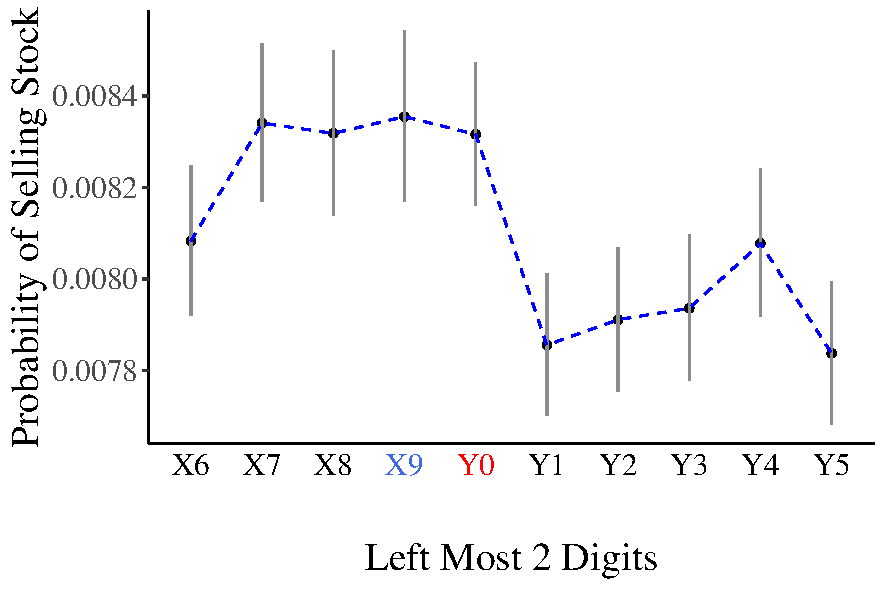
\includegraphics[width=0.45\textwidth]{figures/inc_stock_cross0.pdf}
		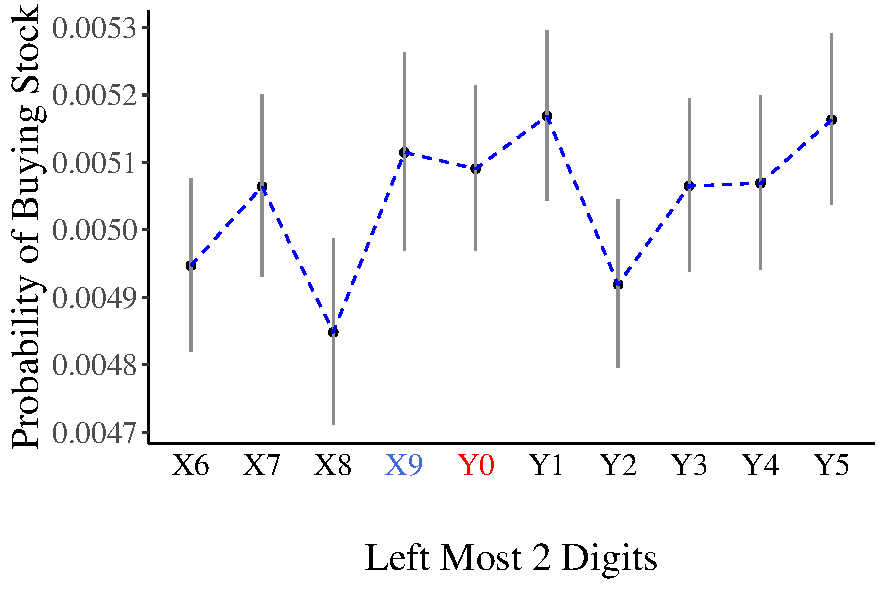
\includegraphics[width=0.45\textwidth]{figures/inc_stock_cross0buy.pdf}
	}
	\subfigure[Stock crosses Y0 and Y5]{
		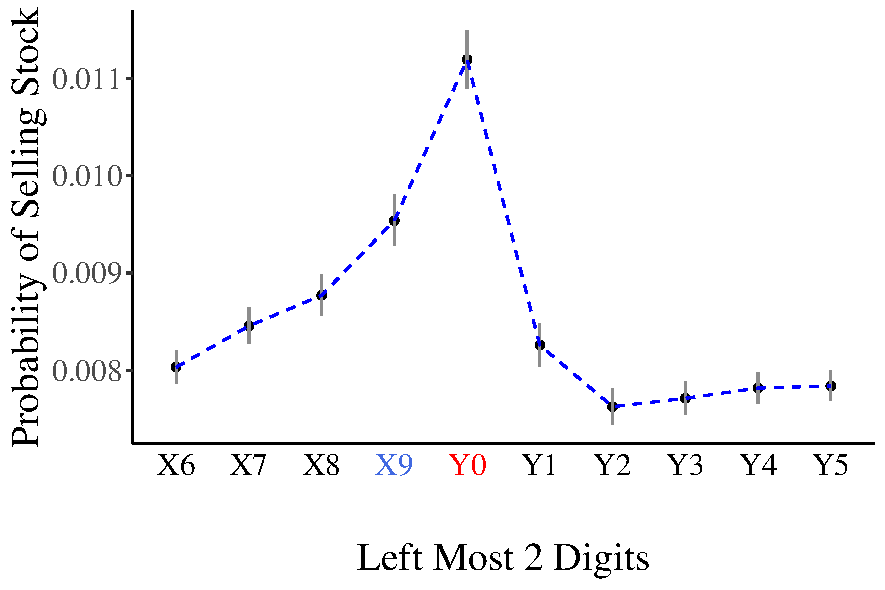
\includegraphics[width=0.45\textwidth]{figures/inc_stock_cross05.pdf}
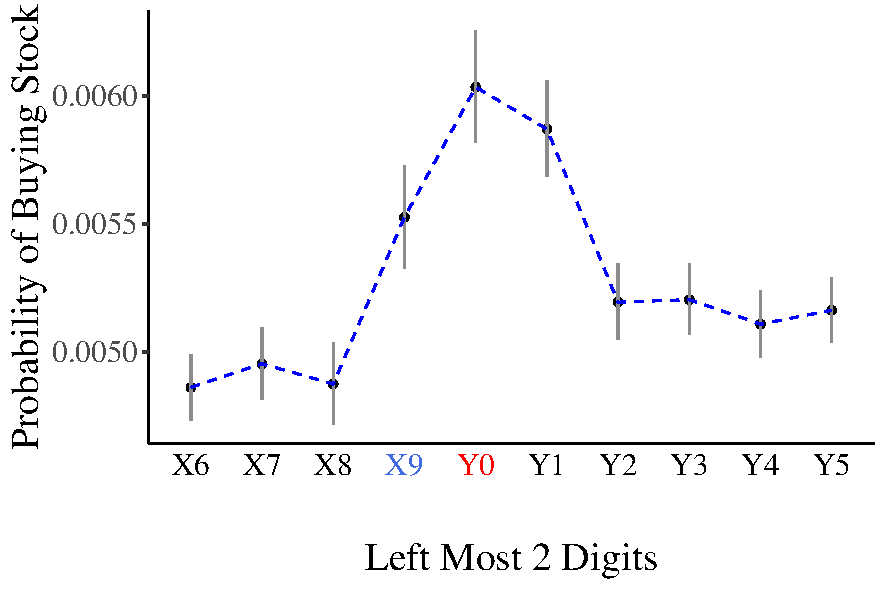
\includegraphics[width=0.45\textwidth]{figures/inc_stock_cross05buy.pdf}
	}

	\fignote{£$Y$ in the X-axes is equivalent to £$X+1$ (e.g., £X9 could include £0.19, £1.9, £19, etc., while £Y0 could include £0.20, £2.0, £20, etc.). }
\end{figure}



\begin{figure}[hbt!]
	\caption{Leftmost Stock Price Digit and Probability of Sale/Buy \\ Prices Decreasing Sample}%
	\label{fig:decreasing}%
	\centering%	
	\bigskip
	\subfigure[Stock crosses Y0 (to X9)]{
		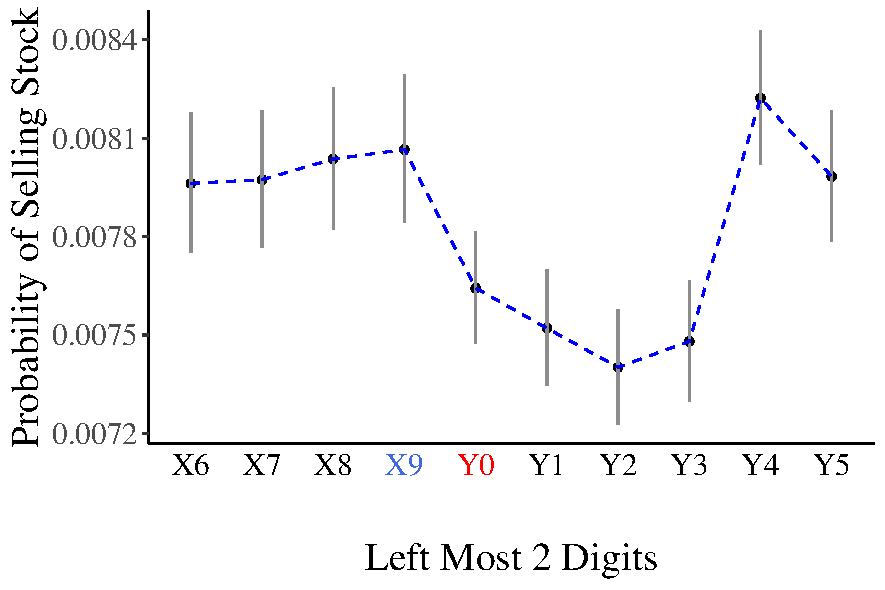
\includegraphics[width=0.45\textwidth]{figures/dec_stock_cross0.pdf}
		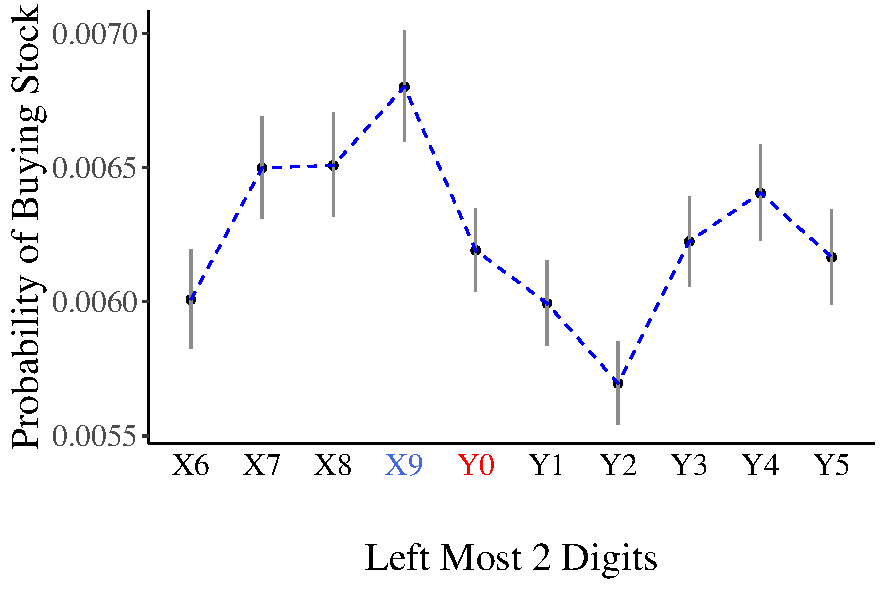
\includegraphics[width=0.45\textwidth]{figures/dec_stock_cross0buy.pdf}
	}
	\subfigure[Stock crosses Y0 and Y5]{
		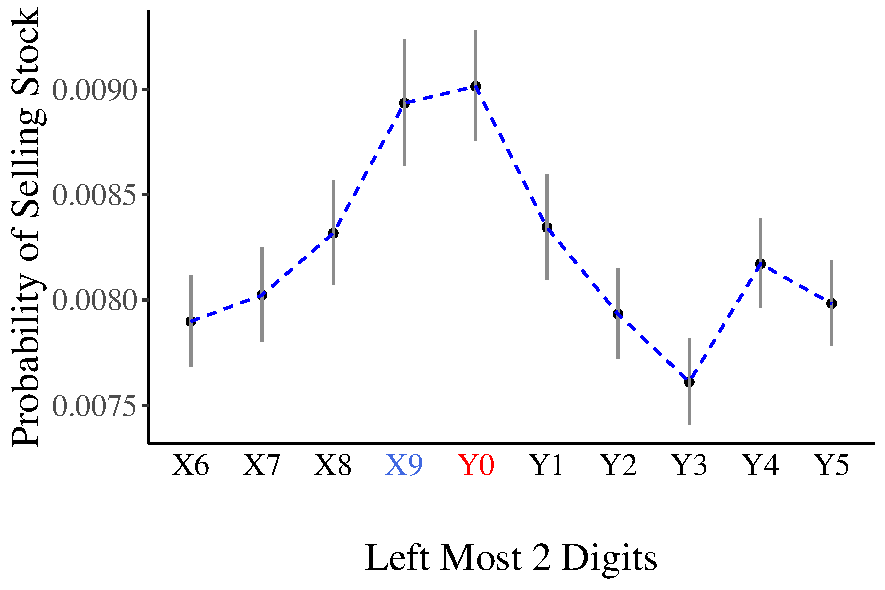
\includegraphics[width=0.45\textwidth]{figures/dec_stock_cross05.pdf}
		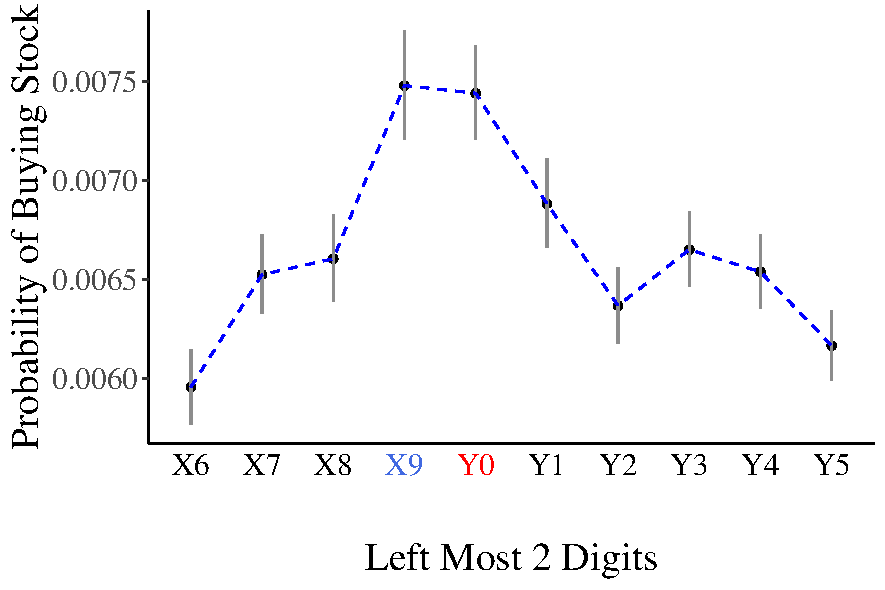
\includegraphics[width=0.45\textwidth]{figures/dec_stock_cross05buy.pdf}
	}
	
	\fignote{£$Y$ in the X-axes is equivalent to £$X+1$ (e.g., £X9 could include £0.19, £1.9, £19, etc., while £Y0 could include £0.20, £2.0, £20, etc.). }
\end{figure}



\begin{figure}[hbt!]
	\caption{Leftmost Stock Price Digit and Probability of Sale/Buy \\ New Sample Criteria \\ \textbf{Days with Changes in Prices and Changes in Second Digits}}%
	\label{fig:new_change_p_digit}%
	\centering%	
	\bigskip
	\subfigure[Price on $t$ > Price on $t-1$ \& Second digit change on $t$]{
		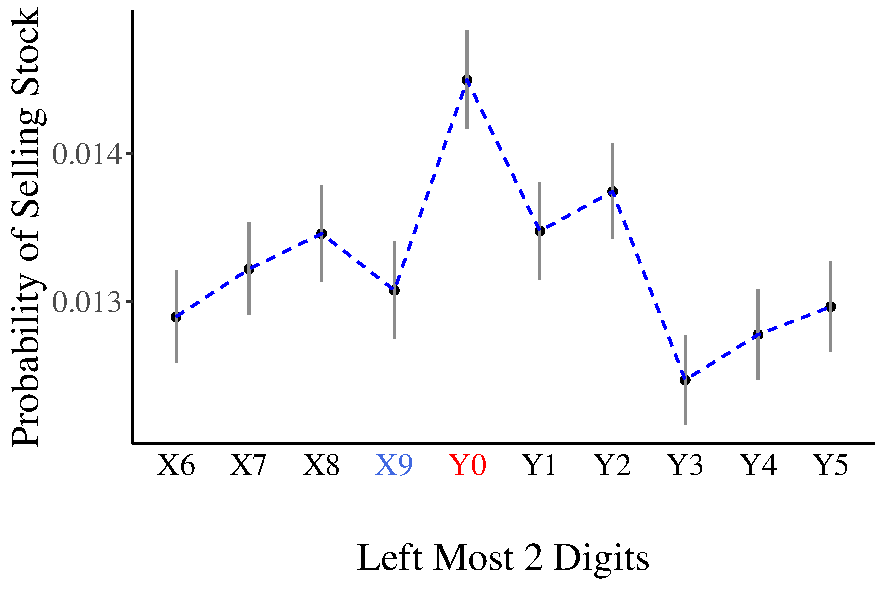
\includegraphics[width=0.45\textwidth]{figures/inc_cond_yest.pdf}
		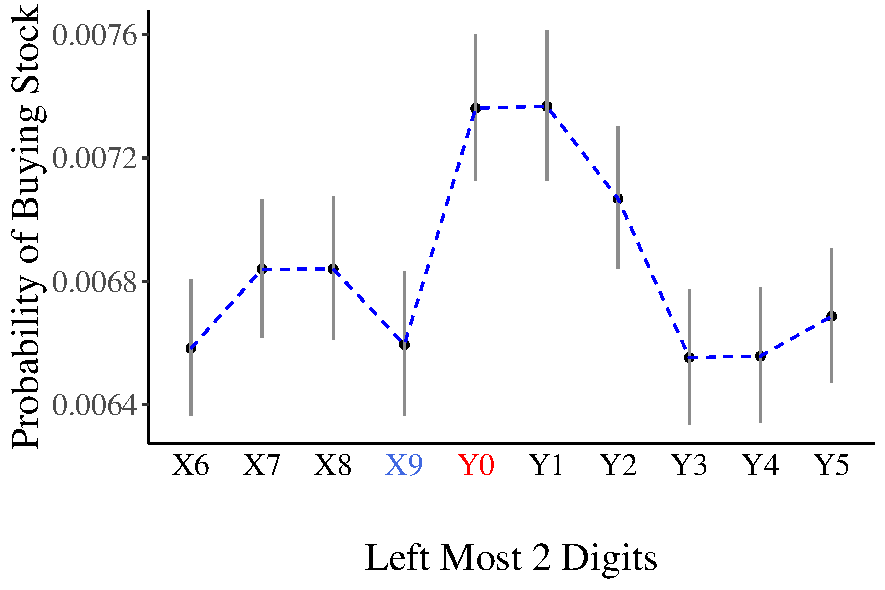
\includegraphics[width=0.45\textwidth]{figures/inc_cond_yest_buy.pdf}
	}
	\subfigure[Price on $t$ < Price on $t-1$ \& Second digit change on $t$]{
		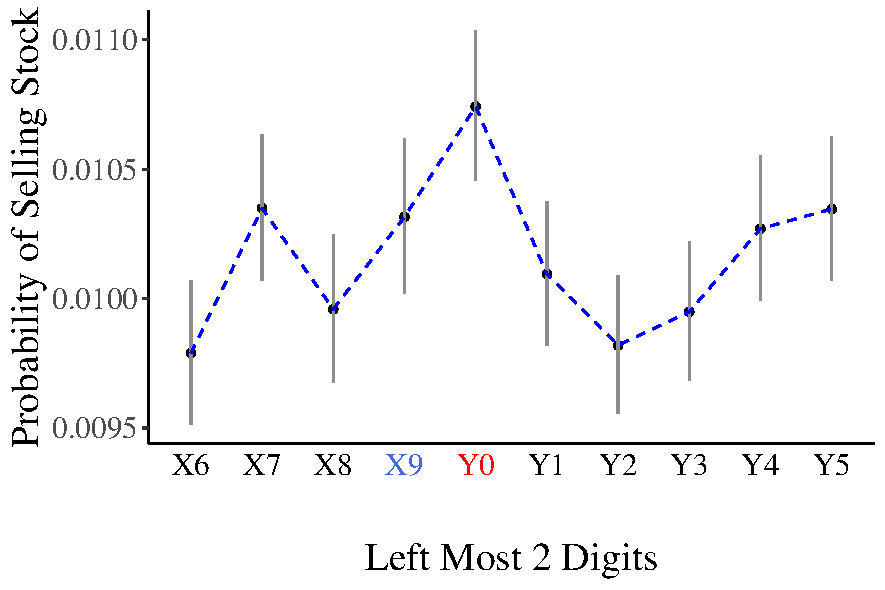
\includegraphics[width=0.45\textwidth]{figures/dec_cond_yest.pdf}
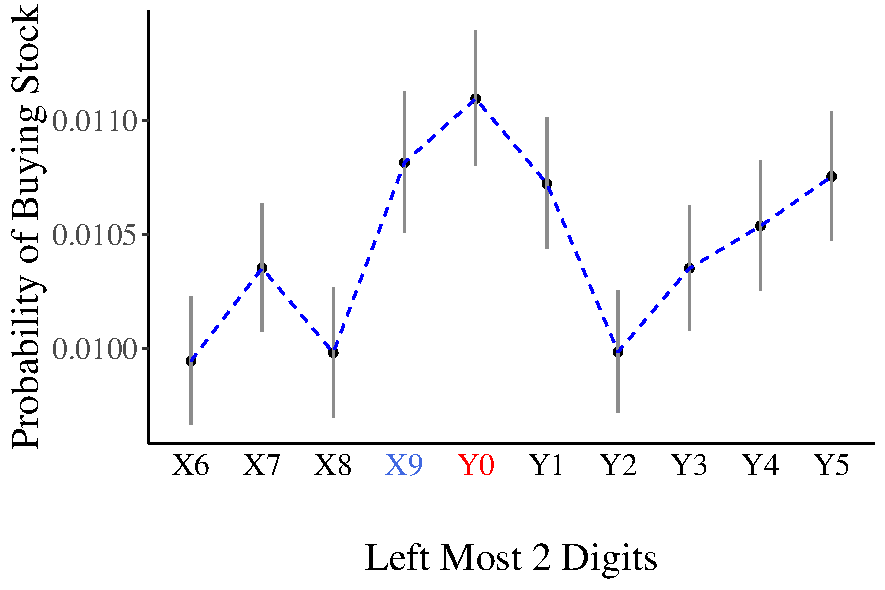
\includegraphics[width=0.45\textwidth]{figures/dec_cond_yest_buy.pdf}
	}
		\subfigure[Price on $t$ != Price on $t-1$ \& Second digit change on $t$]{
		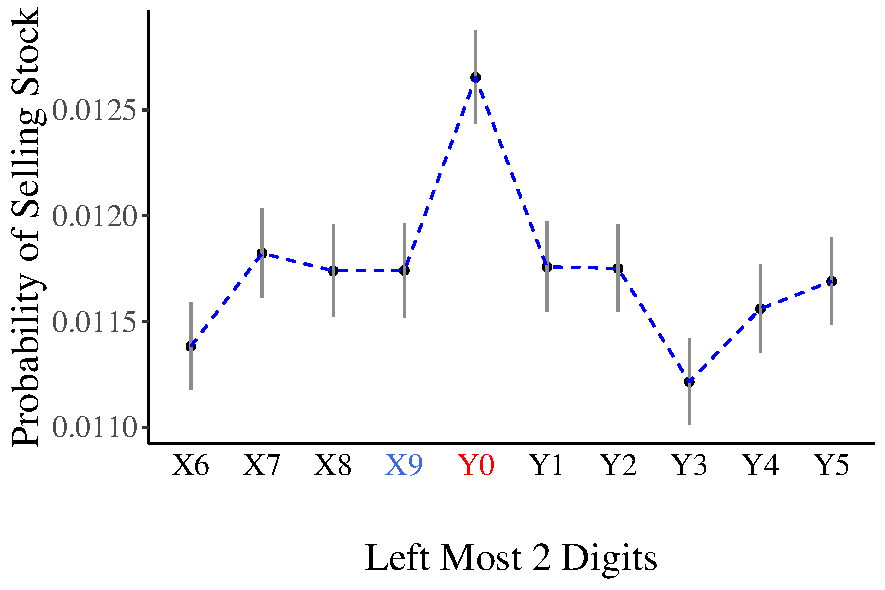
\includegraphics[width=0.45\textwidth]{figures/all_cond_yest_change.pdf}
		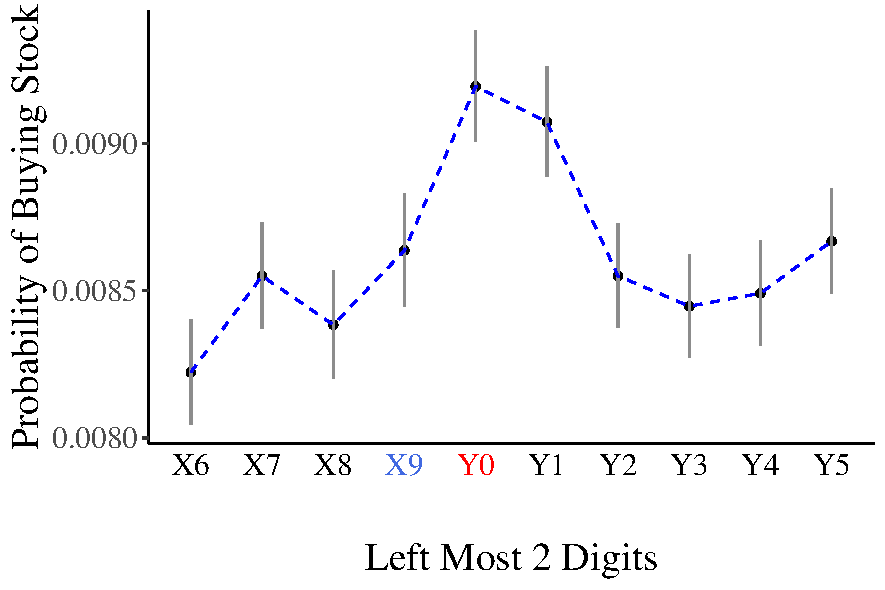
\includegraphics[width=0.45\textwidth]{figures/all_cond_yest_change_buy.pdf}
	}
	\fignote{£$Y$ in the X-axes is equivalent to £$X+1$ (e.g., £X9 could include £0.19, £1.9, £19, etc., while £Y0 could include £0.20, £2.0, £20, etc.). }
\end{figure}


\begin{figure}[hbt!]
	\caption{Leftmost Stock Price Digit and Probability of Sale/Buy \\ New Sample Criteria \\ \textbf{Days with Changes in Prices and Unchanged Second Digits}}%
	\label{fig:new_change_p}%
	\centering%	
	\bigskip
	\subfigure[Price on $t$ > Price on $t-1$ \& Second digit constant on $t$]{
		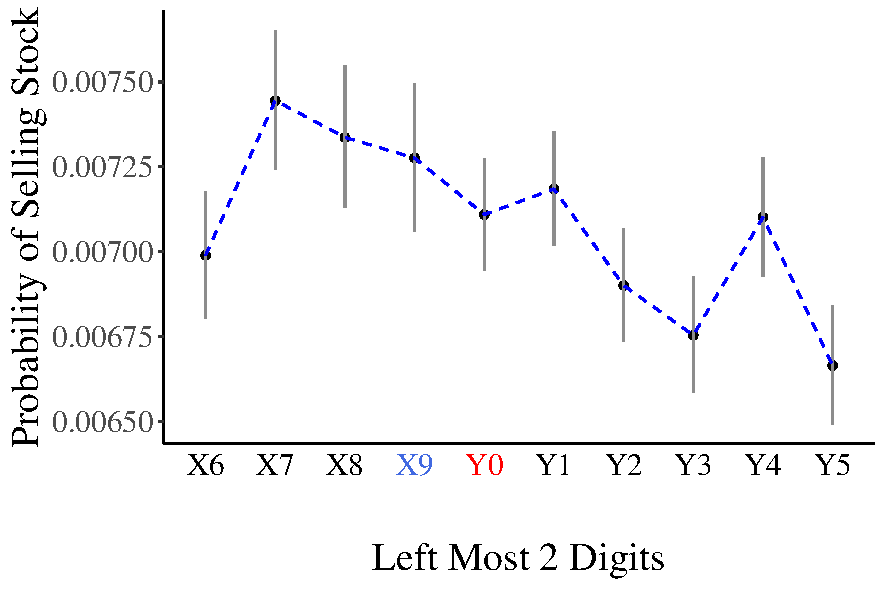
\includegraphics[width=0.45\textwidth]{figures/inc_cond_yest_nochange.pdf}
		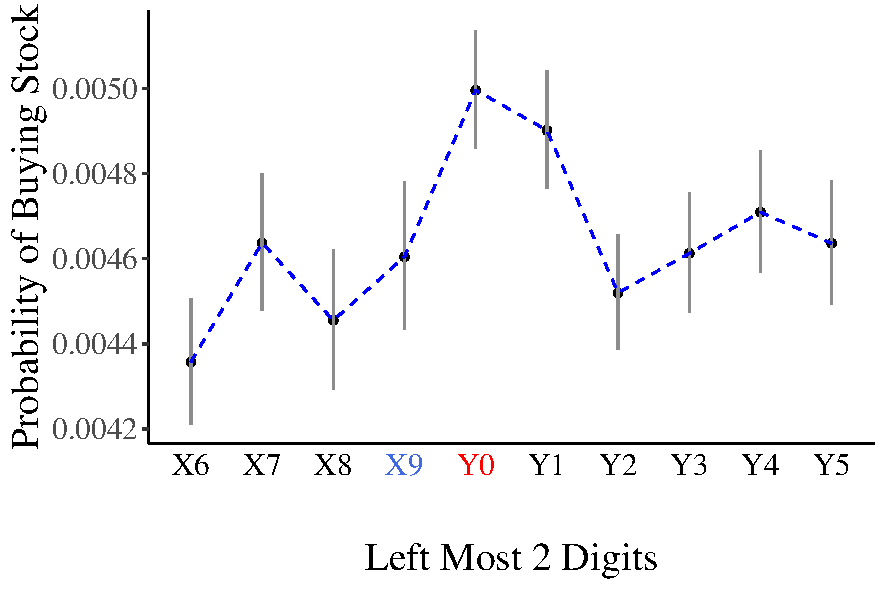
\includegraphics[width=0.45\textwidth]{figures/inc_cond_yest_nochange_buy.pdf}
	}
	\subfigure[Price on $t$ < Price on $t-1$ \& Second digit constant on $t$]{
		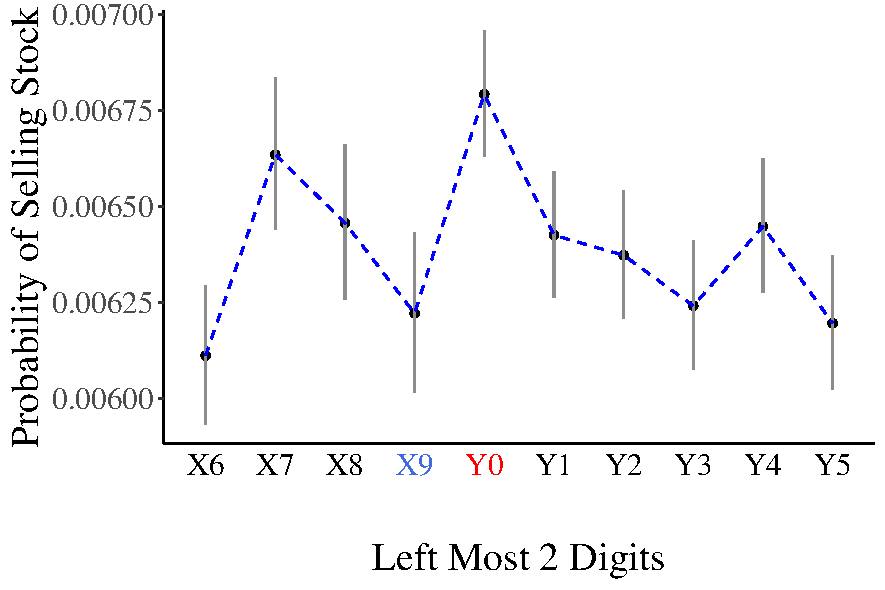
\includegraphics[width=0.45\textwidth]{figures/dec_cond_yest_nochange.pdf}
		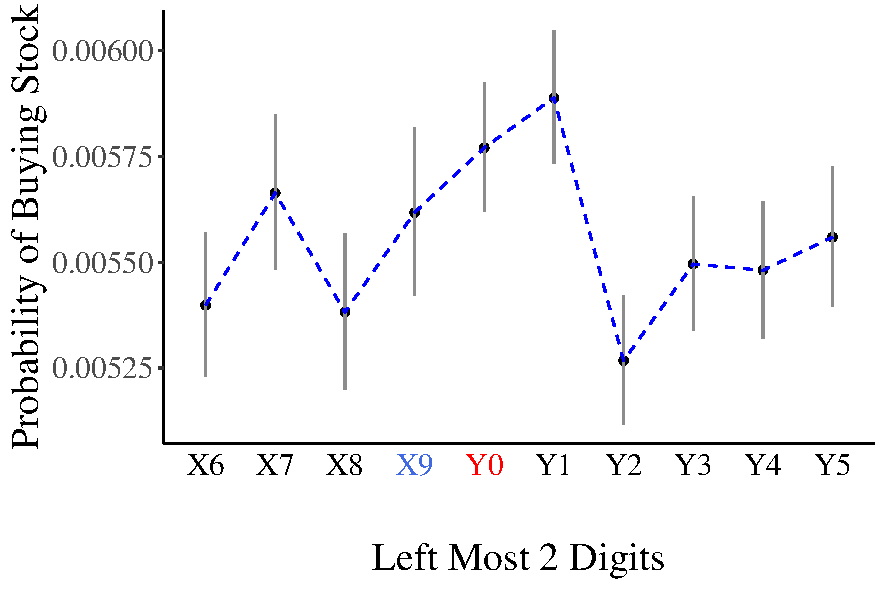
\includegraphics[width=0.45\textwidth]{figures/dec_cond_yest_nochange_buy.pdf}
	}
	\subfigure[Price on $t$ != Price on $t-1$ \& Second digit constant on $t$]{
	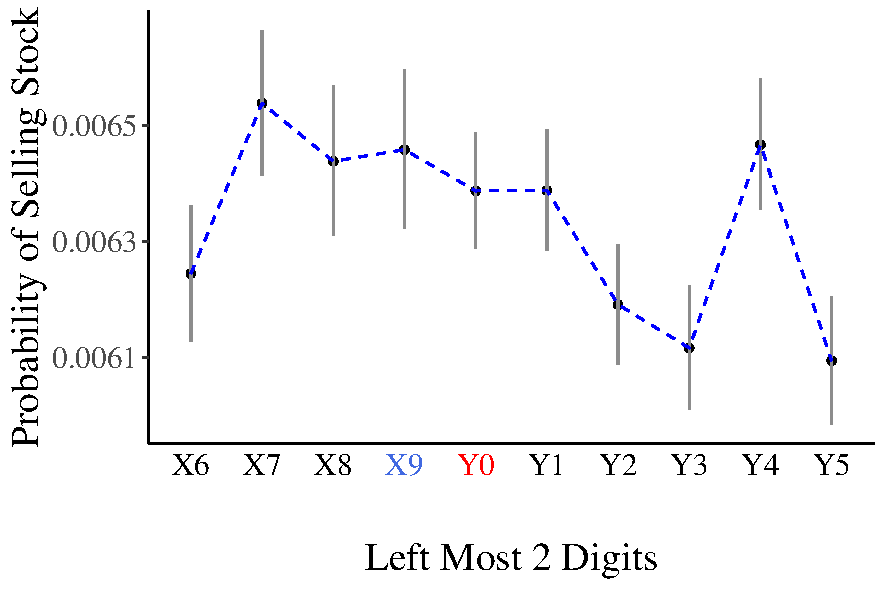
\includegraphics[width=0.45\textwidth]{figures/all_cond_yest_nochange.pdf}
	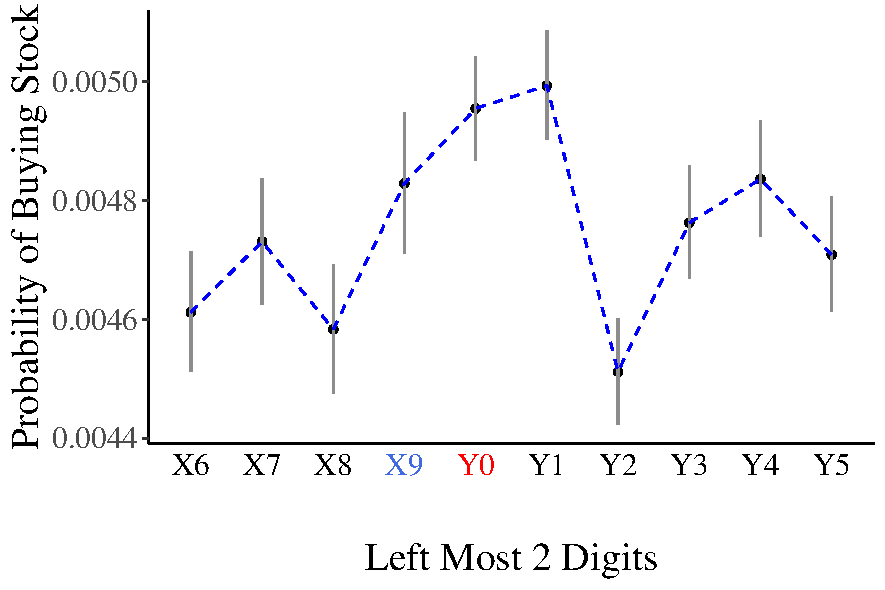
\includegraphics[width=0.45\textwidth]{figures/all_cond_yest_nochange_buy.pdf}
}

	
	\fignote{£$Y$ in the X-axes is equivalent to £$X+1$ (e.g., £X9 could include £0.19, £1.9, £19, etc., while £Y0 could include £0.20, £2.0, £20, etc.). }
\end{figure}


\begin{figure}[hbt!]
	\caption{Leftmost Stock Price Digit and Probability of Sale/Buy \\ New Sample Criteria \\ \textbf{All days}}%
	\label{fig:new_all}%
	\centering%	
	\bigskip
	\subfigure[All days]{
		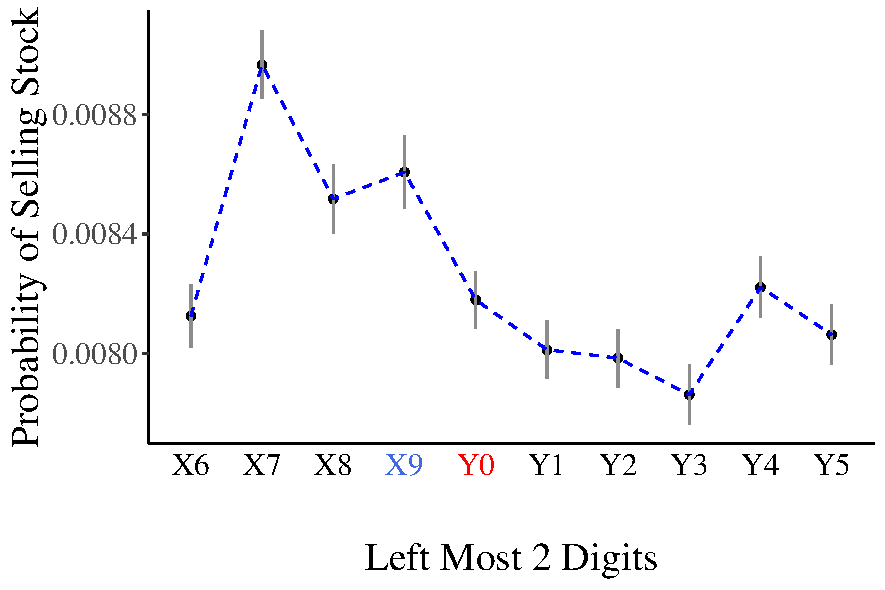
\includegraphics[width=0.45\textwidth]{figures/all_sell.pdf}
		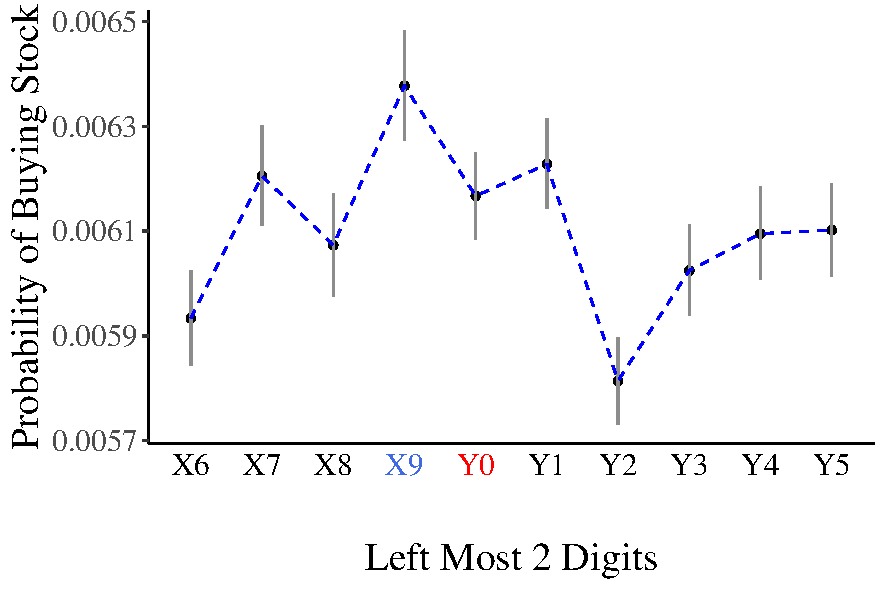
\includegraphics[width=0.45\textwidth]{figures/all_buy.pdf}
	}

	
	
	\fignote{£$Y$ in the X-axes is equivalent to £$X+1$ (e.g., £X9 could include £0.19, £1.9, £19, etc., while £Y0 could include £0.20, £2.0, £20, etc.). }
\end{figure}



\begin{figure}[hbt!]
	\caption{Histograms of Leftmost Stock Price Digit \\ New Sample Criteria} %
	\label{fig:hist}%
	\centering%	
	\bigskip
	\subfigure[Second digit change on $t$]{
		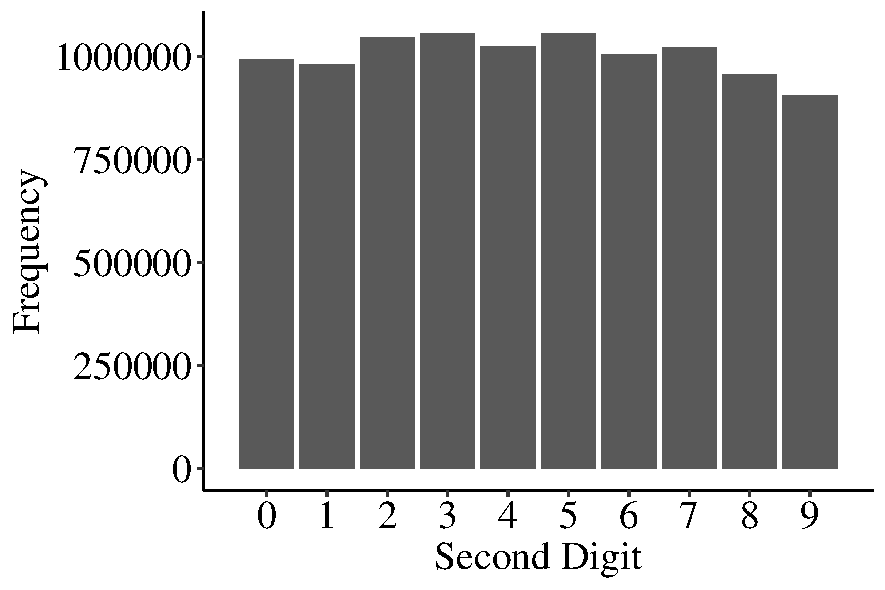
\includegraphics[width=0.55\textwidth]{figures/hist_changedigit.pdf}
	}
	\subfigure[Second digit unchanged on $t$]{
		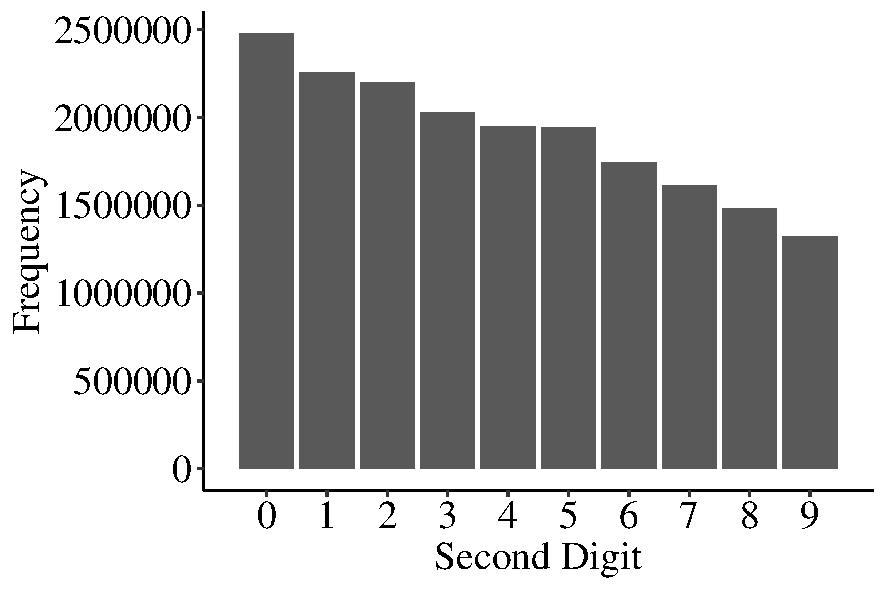
\includegraphics[width=0.55\textwidth]{figures/hist_nochangedigit.pdf}
	}
	\subfigure[All observations]{
		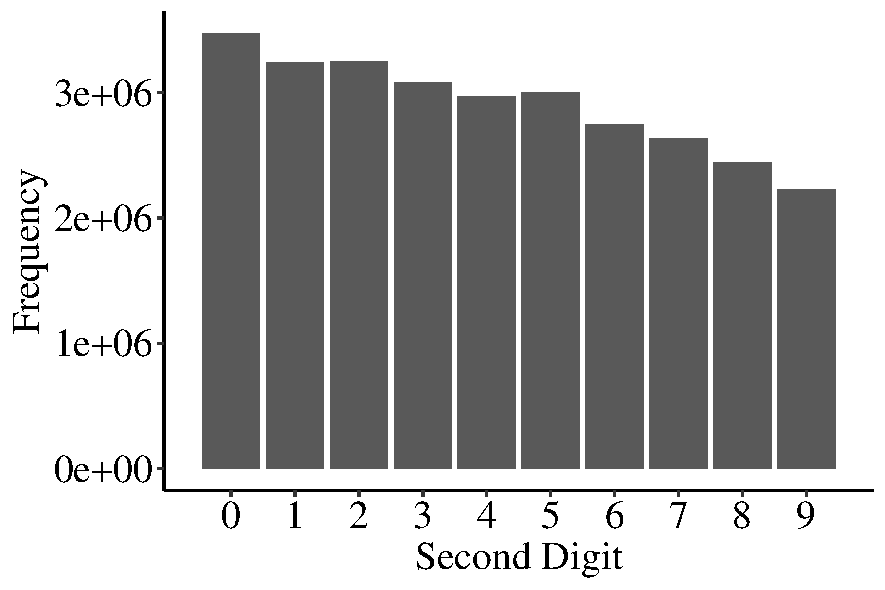
\includegraphics[width=0.55\textwidth]{figures/hist_all.pdf}

	}
	\fignote{}
\end{figure}

\clearpage
\begin{figure}[hbt!]
	\caption{Leftmost Stock Price Digit and Probability of Sale/Buy \\ New criteria (salient changes in price)}%
	\label{fig:salient}%
	\centering%	
	\bigskip
	\subfigure[Price on $t$ > Price on $t-1$ \& Second digit change on $t$ \& Month return > 5\%]{
		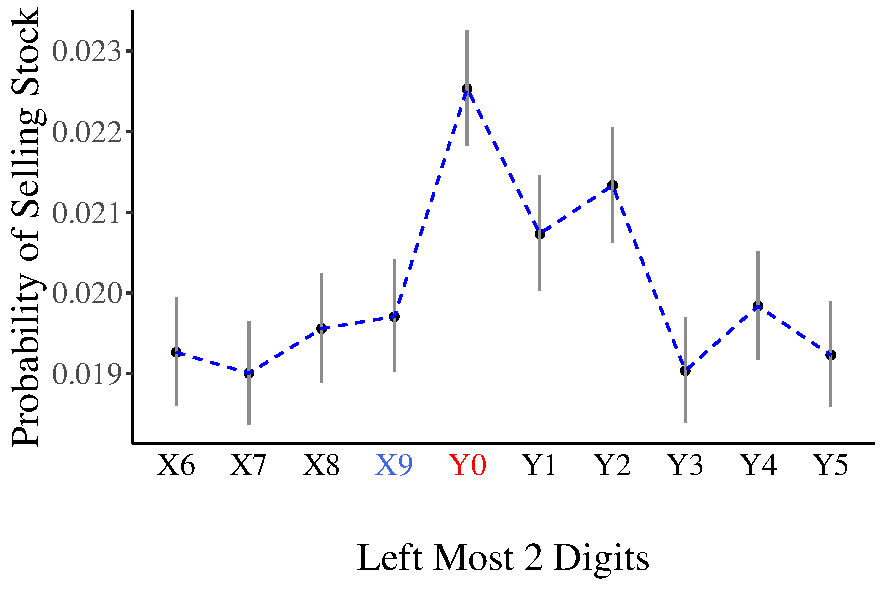
\includegraphics[width=0.45\textwidth]{figures/inc_cond_yest_salient.pdf}
		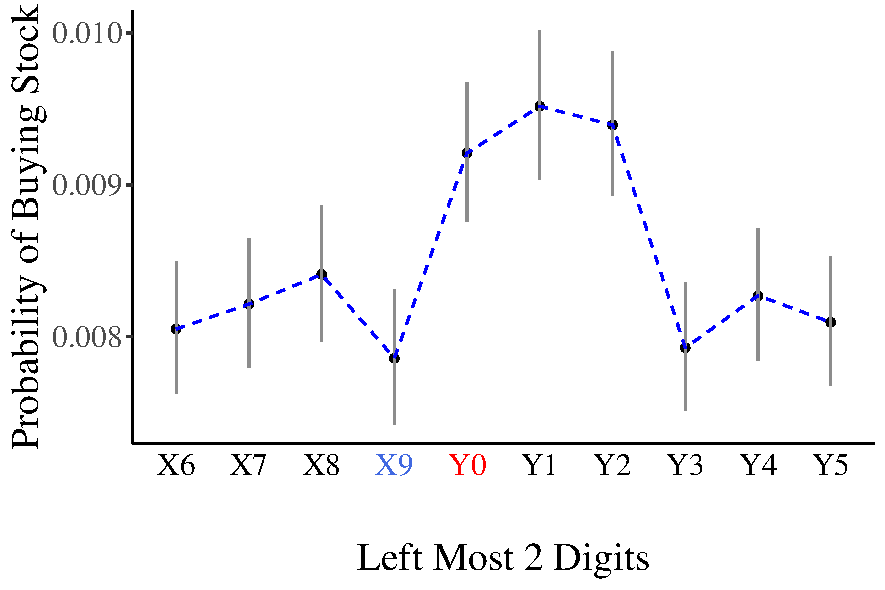
\includegraphics[width=0.45\textwidth]{figures/inc_cond_yest_buy_salient.pdf}
	}
	\subfigure[Price on $t$ < Price on $t-1$ \& Second digit change on $t$ \& Month return < -5\%]{
		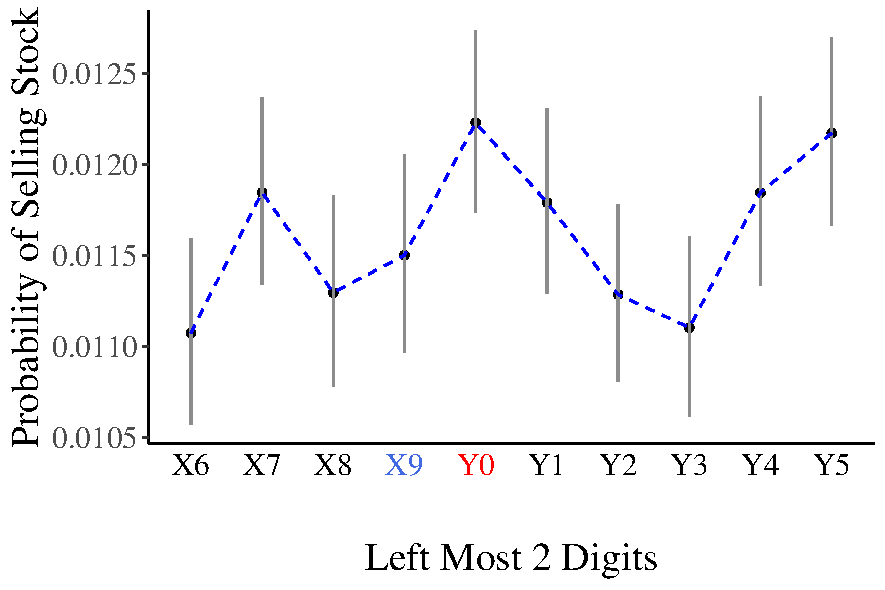
\includegraphics[width=0.45\textwidth]{figures/dec_cond_yest_salient.pdf}
		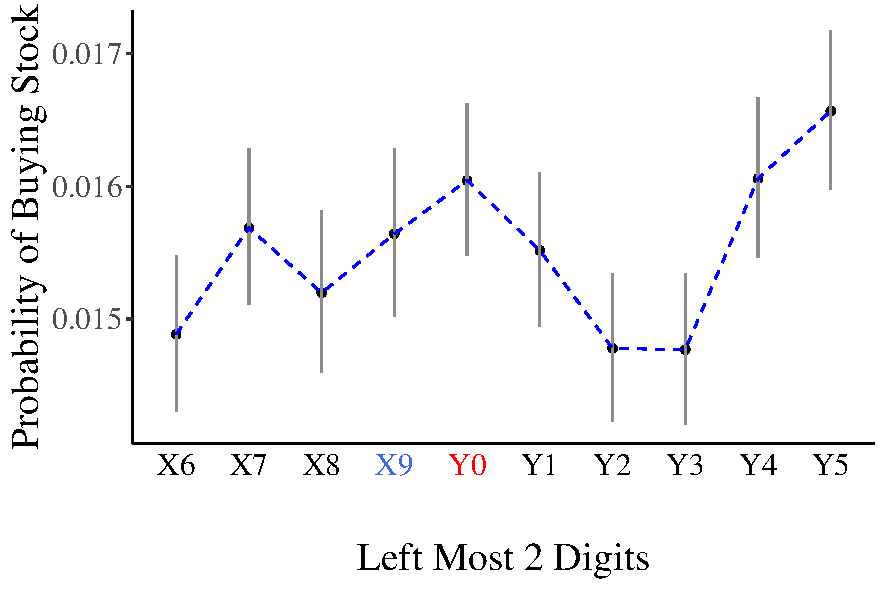
\includegraphics[width=0.45\textwidth]{figures/dec_cond_yest_buy_salient.pdf}
	}
	
	\fignote{£$Y$ in the X-axes is equivalent to £$X+1$ (e.g., £X9 could include £0.19, £1.9, £19, etc., while £Y0 could include £0.20, £2.0, £20, etc.). }
\end{figure}
\end{document}
